\documentclass{beamer}
\usepackage{etex}
\usepackage{amsmath}
\usepackage{beamerthemesplit} % new 
\usepackage{braket}
\usepackage{tikz}
\usepackage{braids}
\usepackage{qcircuit}
\begin{document}
\title{Braids, Jones polynomials and the Phibonacci representation} 
\author{Ohad Barta} 
\date{\today} 

\frame{\titlepage} 
\begin{frame}[allowframebreaks]
\frametitle{Table of contents}
{\tableofcontents}
\end{frame}

\subsection{Knots, Braid groups and Tempely-Lieb Algebra}
\subsubsection{Knots}
\frame{\frametitle{Knots}
A knot is a closed, non-self-intersecting curve that is embedded in three dimensions and cannot be untangled to produce a simple loop (i.e., the unknot). 

\begin{figure}
\centering
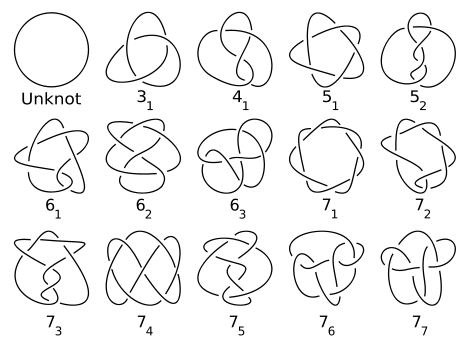
\includegraphics[scale=0.25]{470px-Knot_table}
\caption{Single strand knots}
\label{fig:my_label}
\end{figure}

}

\frame{\frametitle{Knots (2)}
One knot can have multiple strands:
\begin{figure}
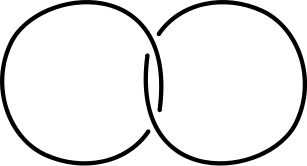
\includegraphics[scale=0.25]{307px-Hopf_link} 
\caption{Hopf link}
\end{figure}
}

\frame{\frametitle{Reidemeister moves}
An old topology question, is to know if two knots are actually the same knot. Reidemeister showed in 1927
the "Reidemeister moves", that do not change the knot.
\begin{figure}
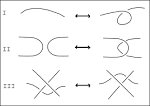
\includegraphics[scale=1]{Reidemeister} 
\caption{Reidemeister moves}
\end{figure}
}
  
\subsubsection{Braid groups}
\frame{\frametitle{Braid groups}
\begin{definition}[Braid]
Consider two horizontal bars, one on top of the other, with $n$-points each. A $n$-strand braid, is
$n$ strands, such that:
\begin{itemize}
\item Each strand has exactly one peg attached to it on each bar
\item The strands may cross one over another
\item At every point on the strand, the strand direction has a non-zero component directed down 
\end{itemize}
\end{definition}
The identity braid:
\begin{center}
\begin{tikzpicture}
\braid[rotate=0,number of strands = 3, style strands={1}{ red } ,style
strands={2}{ blue } ,style strands={3}{ green } ]; 
\end{tikzpicture}
\end{center}

}
\frame{\frametitle{Braid Groups (2)}

We call to the collection of all such braids the braid group \(B_{n}\), with identity element and generators that will immediately follow, when the operation between two braids is put them one below the other, and connect all the bottom-pegs of the first, with the top-pegs of the second.

\begin{center}
\begin{tikzpicture}
\braid[rotate=0, style strands={1}{ red } ,style
strands={2}{ blue } ,style strands={3}{ green } ] s_1 s_1^{-1} 
s_2;
\end{tikzpicture}
\end{center}
 
}

\frame{\frametitle{braid group generators}
\(\forall 1\leq i \leq n\), we denote by \(\sigma_{i}\), the braid which takes the i-th strand
to the (i+1) place, the (i+1)-strand to the i-th place, and leaves all the other strands in place.
For example, this is \(\sigma_{2}\) with 3-strands:
\begin{center}
\begin{tikzpicture}
\braid[rotate=270, style strands={1}{ red } ,style
strands={2}{ blue } ,style strands={3}{ green } ]s_2;
\end{tikzpicture}
\end{center}

Notice that when \(1 < |i - j|\) then \(\sigma_{i}, \sigma_{j}\) act on completely different strands, so they are commutative: \(\sigma_{i}\sigma_{j} = \sigma_{j}\sigma_{i}\)

Furthermore, it holds that \(\sigma_{i}\sigma_{i+1}\sigma_{i} = \sigma_{i+1}\sigma_{i}\sigma_{i+1}\)
(both switch the i-th strand and the (i+2)-strand, while leave all the others in place. See example next slide)
}

\frame{\frametitle{Braid Groups generator rule example}
\begin{center}
\begin{tikzpicture}
\braid[rotate=270, style strands={1}{ red } ,style
strands={2}{ blue } ,style strands={3}{ green } ]s_1 s_2 s_1;
\end{tikzpicture}
\end{center}

\begin{center}
\begin{tikzpicture}
\braid[rotate=270, style strands={1}{ red } ,style
strands={2}{ blue } ,style strands={3}{ green } ]s_2 s_1 s_2;
\end{tikzpicture}
\end{center}


}

\frame{\frametitle{braid groups and knots}
Braids can create a knot by "joining the loose ends" all together. there are two ways of doing it:
The plat closure, where we join neighbour pegs in the top and bottom, and the trace closure, where we connect each top peg to the corresponding bottom peg, without creating more loops.
for example, for the following braid: 

\begin{center}
\begin{tikzpicture}
\braid[rotate=0, height=.3cm, style strands={1}{ red } ,style
strands={2}{ blue } ,style strands={3}{ green } ,style strands={4}{ black } ] s_1 s_2^{-1} 
s_3 s_1 s_2^{-1} s_1^{-1} s_2;
\end{tikzpicture}
\end{center} 

}
\frame{\frametitle{braid groups and knots (2)}
has this closures:
\begin{figure}
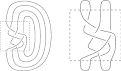
\includegraphics{closures} 
\caption{plat and trace closures}
\end{figure}
}

\subsection{Jones Polynomials} 
\subsubsection{The Kaufmann Bracket Polynomial}
\frame{\frametitle{Jones Polynomials - Introduction}
The jones polynomial matches each knot a polynom , that stays invariant under the Reidemeister moves.
We will first define the Kaufmann Bracket Polynomial, which is "almost" correct.

Consider a knot K. for each crossing in K, from the form 
\begin{center}
\begin{tikzpicture}
\braid[rotate=0, height=.3cm, style strands={1}{ red } ,style
strands={2}{ blue } ] s_1;
\end{tikzpicture}
\end{center} 

We decide at random to replace it with one of two options:
\begin{itemize}
\item The blue strand remains on the right, the red strand remains on the left (choice 1)
\item The blue strand remains on the top, the red strand remains at the bottom (choice 2)
\end{itemize}
Each decision like this for all the crossings is a state \(\sigma\)
}
\frame{\frametitle{The Kaufmann Bracket Polynomial - definition} 
We denote by \(\sigma_{+}\) the number of replaces we made choice 2, and by 
\(\sigma_{-}\) the number of replaces we made choice 1.
We denote by\(N_{\sigma}\) the number of loops created when all the changes of \(\sigma\) are applied.
The Kaufmann Bracket Polynomial is defined as:
\( L(A) = \sum\limits_{all_states_\sigma}{A^{\sigma_{+} -\sigma_{-}}d^{N_{\sigma} - 1}}\)

d is: \(d = -A^{-2} -A^2\) 

}

\frame{\frametitle{The Kaufmann Bracket Polynomial - simple examples}

\begin{itemize}
\item \(\forall A\), L(A)=1 in the unknot:
    \begin{itemize}
    \item we have only one state $\sigma$, with \(\sigma_{+}=0,\sigma_{-}=0\)
    \item this state have one loop, so \(N_{\sigma} = 1\)
    \item Therefore, $L(A) = A^{0}d^{0}=1$
    \end{itemize}
\item For two unknots:
    \begin{itemize}
    \item we have only one state $\sigma$, with \(\sigma_{+}=0,\sigma_{-}=0\)
    \item this state have two loops, so \(N_{\sigma} = 2\)
    \item Therefore, $L(A) = A^{0}d^{1}=d=-A^{-2}-A^{2}$
    \end{itemize}
\end{itemize}
}
\frame{\frametitle{The Kaufmann Bracket Polynomial - simple examples (2)}

\begin{figure}
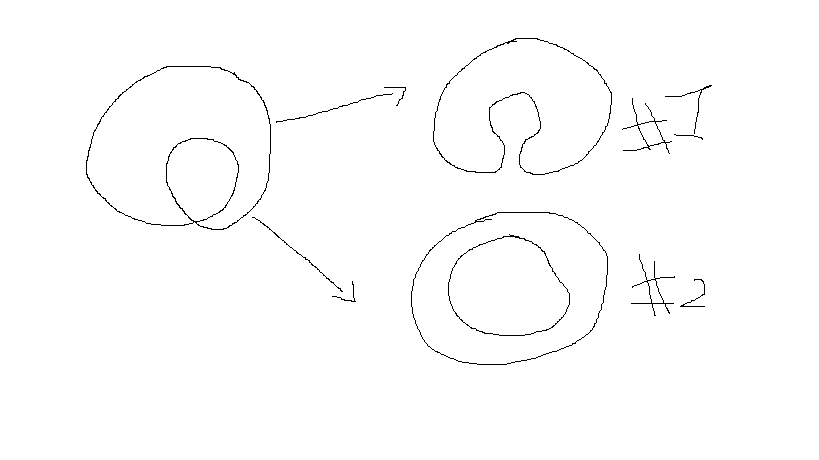
\includegraphics[scale=0.2]{kauffman_calc} 
\caption{kaufmann bracket example}
\end{figure}
:
\begin{itemize}
    \item we have two states. In choice 1, $\sigma_{-}=1$, In choice 2,$\sigma_{+}=1$
    \item If we chooce choice 1 we have \(N_{\sigma} = 1\), if we choose choice 2 we have \(N_{\sigma} = 2\)
    \item Therefore, $L(A) = A^{-1}d^{0} + A^{1}d^{1} = A^{-1} +A^{1}(-A^{-2}-A^{2}) = -A^{3}$
\end{itemize}
}
\frame{\frametitle{recursive formula}
\begin{figure}
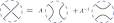
\includegraphics[scale=1]{Kauffman_bracket_identity} 
\caption{kaufmann bracket recursive nature}
\end{figure}
This comes directly from the definition, if we consider only one cross.
\begin{figure}
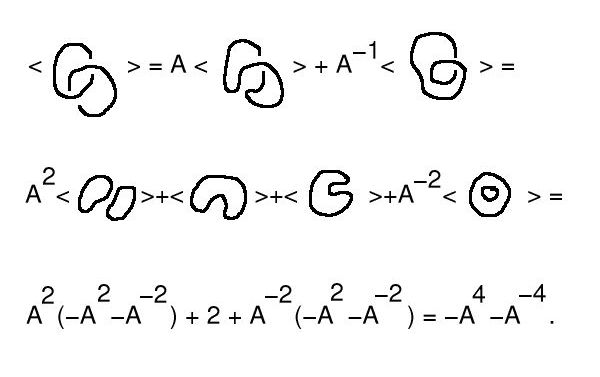
\includegraphics[scale=0.15]{hopf_link} 
\caption{the kaufmann polynomial of the Hopf link}
\end{figure}

\end{itemize}
}

\frame{\frametitle{the connection to Reidiemster moves}
For Completion, we will note that it is easy to see that Jones Polynomial remains the same
under Reidiemster moves. We will show here only one of the three, the others can be proved in a similar technique:
\begin{figure}
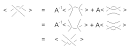
\includegraphics[scale=1]{jones_and_reidimister} 
\caption{the kaufmann polynomial of the Hopf link}
\end{figure}  
}

\subsubsection{The Jones Polynomial}
\frame{\frametitle{The Jones Polynomial definition}
Jones polynomial is different from Kaufmann bracket polynimial only with some normalization factor.
We define by the w(k) for a knot k to be: \(w(k) = \sum\limits_{all crossings}{(-1)^{is the left arrow above the right one}}\)
and Jones polynomial is defines as: \(V_{k}(t)=V_{k}(A^{-4})=(-A)^{3w(k)}L_{k}(A)\).

Notice that w(k) for the unknot is 0, so the Jones polynomial of the unknot is still equals to 1 at any point.
}


\frame{\frametitle{example}
Consider the Hopf link.

Moving to Jones Polynomial, we can see that w(HopfLink)=-2 (two cross with the same oreintation), so:
\(V_{hopfLink}=(-A)^{-6}(-A^{-4}-A^{4}) = -A^{-2} - A^{-10}\).
Remember that \(t = A^{-4}\) and we get \(V_{hopfLink}(t)=-\sqrt{t}(1+t^{2})\)  
}




\subsection{Tempely Lieb-algebra}
\frame{\frametitle{Tempely Lieb algebra}
Tempely Lieb {n,d} algebra group consists of two rows of pegs (button and top), and n-strands, such that:
\begin{itemize}
\item each strand connects to exactly two pegs (but they can be from the same side!)
\item the strands cannot intersect between them.
\item the operator of two objects like this is simply put them one below the other, 
while erasing circuits created, but multiply the final result by d, for each circuit removed
\end{itemize}
\begin{figure}
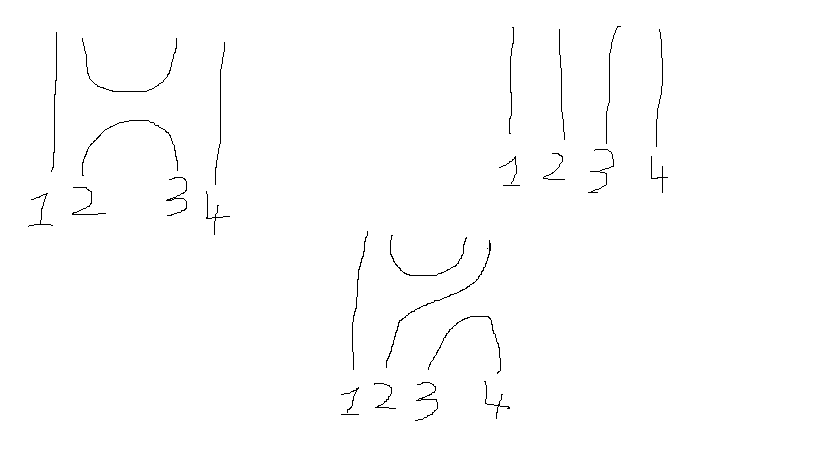
\includegraphics[scale=1]{tempely_lieb_generators} 
\caption{tempely lieb generators}\
\end{figure}

}

\frame{\frametitle{Tempely Lieb algebra generators}
The i-th generator send the ith-strand on the buttom and top the the i+1 peg, 
and leaves all the others in place.

Notice that these generators obeys the following rules 
\begin{itemize}
\item \(E_{i}E_{j} = E_{j}E_{i}\), when \(2 \leq |i-j|\)
\item \(E_{i}E_{i+1}E_{i} = E_{i}\), \(E_{i}E_{i-1}E_{i} = E_{i}\)
\item \({E_{i}}^2 = dE_{i}\)
\end{itemize}


\begin{figure}
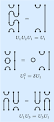
\includegraphics[scale=1]{tempely_lieb_operator} 
\caption{plat and trace closures}
\end{figure}

}

\subsubsection{From braid groups to tempely-lieb algebra }
\frame{\frametitle{From braid groups to tempely-lieb algebra}
 homomorphism from the braid groups to the tempely lied algebra can be defined by its operation on the generators. we will define:
\(\rho_{A}(\sigma_{i}) = AE_{i} +A^{-1}I\), when I is the identity in the lieb-algebra,
and A is a number that satisfies \(A^{2}+A^{-2}=d\).
We can show that this is indeed a representation of the braid groups, if we show that the relations
of the braid group generators still hold (Appears in our full version paper).
}

\subsubsection{The MarkovTrace}
\frame{\frametitle{The Markov Trace}
The Markov Trace is a function on a tempely-Lieb algebra, such that:
\begin{itemize}
\item given a tempely-lieb algebra object, we connect its buttom and top bars, in a similar way to
a trace closure.
\item when denote the number of loops created like this with a, the trace closure is \(d^{a-n}\)
\end{itemize}
\begin{figure}
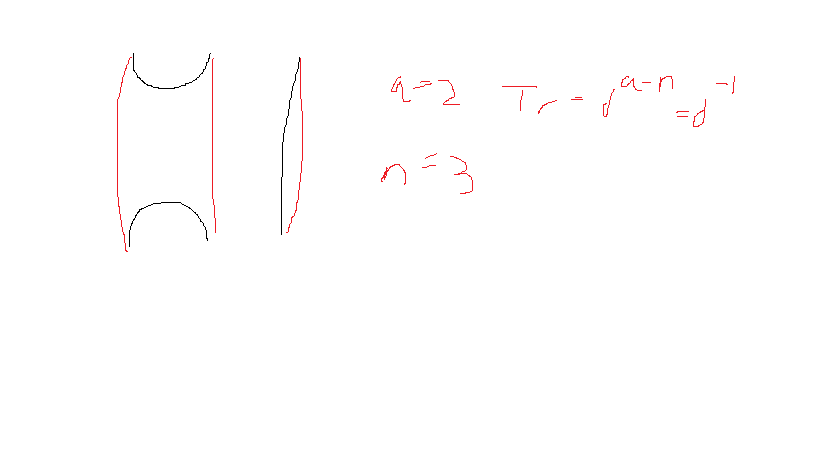
\includegraphics[scale=0.35]{MarkovTraceExample} 
\caption{plat and trace closures}
\end{figure}
}
\frame{\frametitle{The Markov Trace Properties}
The Markov trace Tr obeys the following:
\begin{itemize}
\item Tr[1] = 1 (the identity tempely-algebra has n loops in its clousre, \(d^{n-n} = 1\))
\item \(\forall X,Y \in TL[n,d]\), Tr[XY] = Tr[YX] 
\item \(\forall X \in TL[n-1, d], Tr[xE_{n-1}]=\frac{Tr[x]}{d}\) (add \(E_{n-1}\) add new peg but dont enlarge the number of loops).
\end{itemize}

An important claim (which we prove in the full paper), is that this three properties are enough to uniqely define the value of the markov trace.

}







\frame{\frametitle{the connection to markov trace and braid groups}
We will now show a connection between the Jones Polynomial and the Markov trace.
Proposition:
\(V_{B^{tr}}(A) = (-A)^{3w(B^{tr})}d^{n-1}Tr[\rho_{A}(B)]\)
That is, the Jones polynomial of a trace-closure of some braid is connected to the Markov trace value of its corresponding templely-lieb object.
Proof:

We only have to proof that \(L(B^{tr}) = d^{n-1}Tr[\rho_{A}(B)]\). Recall that for each crossing in the braid B, the kaufmann polynomial hold \begin{figure}
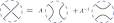
\includegraphics[scale=1]{Kauffman_bracket_identity} 
\caption{kaufmann bracket recursive nature}
\end{figure}.
The homomorphism also has the form of  \(\rho_{A}(\sigma_{i}) = AE_{i} +A^{-1}I\) - exactly the same!.
}
\frame{\frametitle{the connection to markov trace and braid groups(2) }
After choosing a state \(\sigma\), its value in the Kaufmann polynimial is \(d^{(N_{\sigma} -1)}\), and its
value i the Markov trace is \(d^{(N_{\sigma} -n )}\), therefore we need the \(d^{n-1}\) factor. 
 
}
\subsection{The fibonacci representation}
\frame{\frametitle{The fibonacci representation of a braid group}
We would like to obtain some matrix representation of a braid. Given an n-strand braid, we can write a string of n+1 elements on the buttom of the braid between every two strands, where each element is either * or p. The only restriction is that there will be no two adjacent * elements. The number of possibilities to do so is of course \(f_{n+3}\), where \(f_{n}\) denotes the n-th fibonacci number.

Next, for each crossing and labelling of it (the 3 elements from the right, left, and in the crossing) , we would like to give a linear function that will "open up" the crossing, and that may change the center label. (we wouldn't want to change the right or left label, in order to preserve the string of elements correctness under all the operations).
} 

\frame{\frametitle{The fibonacci representation of a braid group (2)}
That is, in the most general form, a cross \(\sigma_{i}\) with labeling of P*P, can move to 
a times * Identity with labelling P*P + b times the identity with labelling PPP.
we will denote it by \((p\hat{*}p)=a(p*p)+b(ppp)\)


Such matrix representation must have some properties that will make it usefull to us:
\begin{itemize}
\item for every braid, its matrix must be unitary, so we can link it to some quantom circuit.
\item for every braid, there has to be some connection between the Jones Polynomial of the braid, and the relevant matrix.
\end{itemize}
} 


\frame{\frametitle{The fibonacci representation of a braid group (3)}
The explicit representation is:
\((*\hat{p}p)=a(*pp)\)

\((*\hat{p}*)=b(*p*)\)

\((p\hat{*}p)=c(p*p)+d(ppp)\)

\((p\hat{p}*)=a(pp*)\)

\((p\hat{p}p)=d(p*p)+e(ppp)\)

, with:
\( a = -A^{4} \)


 \(  b = A^{8}  \)
 
 \(  c = A^{8}\tau^{2} - A^{4}\tau \)
  
 \(  d = A^{8}\tau^{\frac{3}{2}} + A^{4}\tau^{\frac{3}{2}} \) 
 
 \(  e = A^{8}\tau - A^{4}\tau^{2} \) 
 
 \(  A = e^{\frac{-3{\pi}i}{5}} \) 
 
 \(  \tau = \frac{2}{1 + \sqrt{5}} \)


} 
\frame{\frametitle{The Fibonacci representation - example}
We will show the Fibonacci representation of $\sigma_{1}$ with 3 strands:
\[
\begin{pmatrix} b & 0 & 0 & 0 & 0 & 0 & 0 & 0 \\ 0 & a & 0 & 0 & 0 & 0 & 0 & 0 \\ 0 & 0 & a & 0 & 0 & 0 & 0 & 0 \\ 0 & 0 & 0 & e & 0 & d & 0 & 0 \\ 0 & 0 & 0 & 0 & a & 0 & 0 & 0 \\ 0 & 0 & 0 & d & 0 & c & 0 & 0 \\0 & 0 & 0 & 0 & 0 & 0 & e & d \\0 & 0 & 0 & 0 & 0 & 0 & d & c \end{pmatrix} 
  \begin{pmatrix} *p*p \\ *ppp \\ *pp* \\ pppp \\ pp*p \\ p*pp \\ ppp* \\ p*p* \end{pmatrix}
\]
}
\subsubsection{unitarity}
\frame{\frametitle{The Unitary of the Fibonacci representation}
Its enough to prove that all the braid group generators, since multiplication of unitary matrices is again unitary matrix. Each generator like this include only one cross. As we saw in the definition and examples, each cross leaves only 1-2 non-zero elements in each matrix row, in the corresponding labelling entry.

we will move onto the 5 options to label the 3 elements near the cross (since the other elements doesnt matter here).
\begin{itemize}
\item with all the labelling with the form ...*pp... , the unitary row will include only one "a" in the matrix diagonal, and no other row have non-zero entries in that column. That is, with multiplied by its dagger, the entry on the diagonal will be \(a^{\dagger}a = e^{\frac{-12{pi}i}{5}}e^{\frac{12{pi}i}{5}} = 1\), and all the other entries will be zero.
\item the same reasoning apply to all the other rows combination (full proof is include in the paper)  
\end{itemize}
}

\subsubsection{Fibonacci representation and Jones Polynomial}
\frame{\frametitle{Fibonacci representation and Jones polynimial}
We will want to connect somehow between the Fibonacci representation and the Jones Polynomial\cite{SJ2008}.
For this, we will use the Tempely Lieb algebra, and the Markov Trace. We saw that the Markov trace
is a uniquely defined function over the Tempely-Lieb algebra, such that it is strongly connected to the Jones Polynomial. If we will be able to define a function over the Fibonacci representation that "behaves the same", we will be able to show such correlation between Jones Polynomial and the Fibonacci representation. We will donate this function as \(\tilde{Tr}\)
}

\frame{\frametitle{Fibonacci representation and Jones polynimial (2)}
The requirements from  \(\tilde{Tr}\) are:
\begin{itemize}
\item \(\tilde{Tr}(1) = 1\)
\item \(\tilde{Tr}(XY) = \tilde{Tr}(YX)\)
\item  \( \tilde{Tr}[xE_{n-1}]=\frac{\tilde(Tr)[x]}{d}\)    
\end{itemize}
The last requirement, however, regards to a specific Templerly-Lieb element. Thus, we have to show that the Fibonacci representation and the Temperly-Lieb algebra "live in the same world", in order to translate \(E_{n-1}\) to some matrix in the Fibonacci representation, and prove the requirement on the matrix after the translation. Therefore, in order to even start talking on \(\tilde{Tr}\), we have to show a representation of the Temperly-Lieb algebra inside the Fibonacci representation.  
}

\frame{\frametitle{Fibonacci representation and Jones polynimial (3)}
The requirements from the representation, are, as always, to preserve the original generators properties.
Here, the representation is: \(\rho_{b}(E_{i}) = A^{-1}\rho_{F}(\sigma_{i}) - A^{-2}1\) , with 1 symbols the identity matrix.

it should hold that:
\begin{itemize}
\item \(\rho_{b}(E_{i})\rho_{b}(E_{j}) = \rho_{b}(E_{j})\rho_{b}(E_{i}), when 2 \leq |i-j|\).This hold, since the Fibonacci representation is a representation, so \(\rho_{F}(\sigma_{i}),\rho_{F}(\sigma_{j})\) commutes, and therefore \(\rho_{b}(E_{i}),\rho_{b}(E_{j})\) commutes.
\item  \({\rho_{b}(E_{i}}^{2}) = d\rho_{b}(E_{i})\) : in a similar way to what we did in the unitary proof, we can divide each  \(\rho_{F}(\sigma_{i})\) to blocks of
\[
\begin{pmatrix} a \end{pmatrix}
\begin{pmatrix} b \end{pmatrix}
\begin{pmatrix} c & d \\ d & e \end{pmatrix}
\], and prove that this relation hold on each block separately.  
\end{itemize}
}


\frame{\frametitle{Fibonacci representation and Jones polynimial (4)}
The last requirement we should prove is that  
 \(\rho_{b}(E_{i})\rho_{b}(E_{i+1})\rho_{b}(E_{i}) = \rho_{b}(E_{i})\))
 . Direct calculation shows that \(rho_{b}(E_{1}), rho_{b}(E_{2})\) with 3 strands satisfy this requirement. This suffice, since the relation between \rho_{b}(E_{i}), \rho_{b}(E_{i+1})\) remains the same when i is change (up to re-index of the matrix, the matrix doesn't change), or when the number of strands get bigger with the same index (we will have more "squares" of the form mentioned in the previous slide for more equivalent labellings).
}

\frame{\frametitle{Fibonacci representation and Jones polynimial (5)}
Its time to consider the specific function \(\tilde{Tr}\), and prove its desired properties.
\(\tilde{Tr}\) Definition:


\(\tilde{Tr} = \frac{1}{{\phi}f_{n}+f_{n-1}}\sum\limits_{s \in Q_{n+1}}{W_{s}}\rho_{f}(b)_{s,s}\),
when \(\rho_{f}(b)_{s,s}\) denote the s-th diagonal entry in the Fibonacci representation of b,
and \(W_{s}\) is \(\phi\)if s ends with p, and 1 if s ends with *. \(Q_{n+1}\) is the set of all strings with length n+1 that obeys the "no two adjective *" rule. 

}

\frame{\frametitle{Fibonacci representation and Jones polynimial (6)}
Its easy to see that \(\tilde{Tr}(1) = 1\). In the identity matrix, all the diagonal entries equals to one, there are \(f_{n}\) entries that end with p, and \(f_{n-1}\)entries that end with *, so 
\(\tilde{Tr} = \frac{1}{{\phi}f_{n}+f_{n-1}}\sum\limits_{s \in Q_{n+1}}{W_{s}}\rho_{f}(b)_{s,s} =
 \frac{1}{{\phi}f_{n}+f_{n-1}} ({\phi}f_{n}+f_{n-1}) = 1\)
 
 
 Its easy to see that \(\tilde{Tr}(XY) = \tilde{Tr}(YX)\), since at the end we talking about traces of matrices, and trace is a commutative property.
}

\frame{\frametitle{Fibonacci representation and Jones polynimial (6)}


We remain with the last requirement of  \( \tilde{Tr}[xE_{n-1}]=\frac{\tilde(Tr)[x]}{d}\) . First, we will instantiate \(E_{n-1}\) according to its representation: \(E_{n-1} = A^{-1}\rho_{F}(\sigma_{n-1}) - A^{-2}1\). Therefore, \( \tilde{Tr}[xE_{n-1}] = \tilde{Tr}[A^{-1}x\rho_{F}(\sigma_{n-1}) - A^{-2}x]\)

Therefore, from the linearity of the trace we get  \( \tilde{Tr}[xE_{n-1}] = A\tilde{Tr}[{\rho_{f}({\rho_{f}}^{-1}(x) * \sigma_{n-1})}] -A^{-2}\tilde{Tr}[x]\)

Therefore, it remain to check  the value of \(\tilde{Tr}[{\rho_{f}({\rho_{f}}^{-1}(x) * \sigma_{n-1})}]\)

A careful examination of all the different labelling options of the new strand, combined with the Fibonacci representation rules for the new crossing, yield that this requirement indeed hold
}
\section{References}
\frame{\frametitle{References}
\begin{thebibliography}{9}

\bibitem{SJ2008}
   Peter W. Shor,
   Stephen P. Jordan,
  Estimating Jones Polynomials is a Complete Problem for One Clean Qubit,
   2008.

\bibitem{DVZ2006}
   Dorit Aharonov,
   Vaughan Jones,
   Zeph Landau,
  A Polynomial Quantum Algorithm for Approximating the Jones,
   2006.
\end{thebibliography}
}
\end{document}